% !TeX program = xelatex
% !TeX encoding = utf8
% !TeX root = RegT1E_HS22.tex

%% TODO: publish to CTAN
\documentclass[margin=normal]{tex/hsrzf}

%%%%%%%%%%%%%%%%%%%%%%%%%%%%%%%%%%%%%%%%%%%%%%%%%%%
% Packages
\usepackage{mutlicol}
\usepackage[export]{adjustbox}
\usepackage{bm}
%% TODO: publish to CTAN
\usepackage{tex/hsrstud}

%% Language configuration
\usepackage{polyglossia}

\setdefaultlanguage[variant=swiss]{german}

%% License configuration
\usepackage[
    type={CC},
    modifier={by-nc-sa},
    version={4.0},
    lang={german},
]{doclicense}


%%%%%%%%%%%%%%%%%%%%%%%%%%%%%%%%%%%%%%%%%%%%%%%%%%%
% Metadata

\course{Elektrotechnik}
\module{RegT1E}
\semester{Herbstsemester 2022}

\authoremail{joel.leirer@ost.ch}
\author{\textsl{Joël Leirer} -- \texttt{\theauthoremail}}

% did someone help you with this work?
\contributors{
  % I created this template, does that count?
  Naoki Pross
  % do not forget to add yourself!
}

\title{\texttt{\themodule} Zusammenfassung}
\date{\thesemester}

%%%%%%%%%%%%%%%%%%%%%%%%%%%%%%%%%%%%%%%%%%%%%%%%%%%
% Document

\begin{document}

% use roman numberals for introductiory pages
\pagenumbering{roman}

\maketitle


% show the names of the people who contributed to this document.
% \section*{Contributors}
% \thecontributors

\section*{Lizenz}
\doclicenseThis

\clearpage
\tableofcontents

% actual content
\clearpage
\setcounter{page}{1}
\pagenumbering{arabic}

%%%%%%%%%%%%%%%%%%%%%%%%%%%%%%%%%%%%%%%%%%%%%%%
%Includes + Defines
%%%%%%%%%%%%%%%%%%%%%%%%%%%%%%%%%%%%%%%%%%%%%%

%\usepackage{color, colortbl}
%\usepackage{trfsigns}
%\usepackage{graphicx}
%\usepackage{adjustbox}
%\definecolor{TabularBackgroundColor}{rgb}{0.83,0.96,0.96}


%%%%%%%%%%%%%%%%%%%%%%%%%%%%%%%%%%%%%%%%%%%%%%
%Content
%%%%%%%%%%%%%%%%%%%%%%%%%%%%%%%%%%%%%%%%%%%%%%

\section{Wichtige Funktionen}

\small

\subsubsection*{Diracimpuls \tiny (auch Impuls-/Deltafunktion,-Distribution)}

\begin{multicols}{2}

  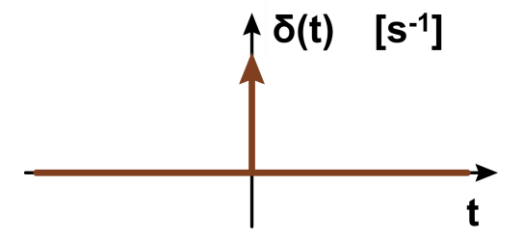
\includegraphics[width = 5cm]{include/Wichtige Funktionen/img/Impulsfunktion.png}

  {\footnotesize
    Unendlich kurzer, normierter Impuls mit unendlicher Amplitude. }

  \resizebox{0.5\textwidth}{!}{%
    \begin{tabular}{ccl}
      \hline \rowcolor{TabularBackgroundColor}
      1.  & $\delta(-t) = \delta(t) $                                                                                            & gerade Funktion                        \\
      \hline
      2.  & $\delta(-t+t_0) = \delta(t-t_0)$                                                                                     & symmetrisch                            \\
      \hline \rowcolor{TabularBackgroundColor}
      3.  & $\delta(at)= \frac{1}{|a|}\delta(t)$                                                                                 & Skalierung                             \\
      \hline
      4.  & $\delta(\frac{t-t_0}{a}) = |a| \cdot \delta(t-t_0)$                                                                  & Skalierung und Verschiebung            \\
      \hline \rowcolor{TabularBackgroundColor}
      5.  & $\delta(t-t_0)f(t) = f(t_0)\delta(t-t_0)$                                                                            & Abtastung                              \\
      \hline
      6.  & $\int \limits _{-\infty} ^{\infty} \delta(t-t_0)f(t)dt = f(t_0)$                                                     & Siebungseigenschaft                    \\
      \hline \rowcolor{TabularBackgroundColor}
      7.  & $\int \limits _{-\infty} ^{\infty}  A\cdot \delta(t)dt = A$                                                          & Spezialfall Siebungseigenschaft        \\
      \hline
      8.  & $\delta(t-t_0) * f(t) = f(t-t_0)$                                                                                    & Faltung                                \\
      \hline \rowcolor{TabularBackgroundColor}
      9.  & $\delta(t-t_1) * \delta(t-t_2) = \delta(t-t_1-t_2)$                                                                  & Faltung                                \\
      \hline
      10. & $\delta(t) = \frac{du(t)}{dt}$                                                                                       & Ableitung Einheitssprung               \\
      \hline \rowcolor{TabularBackgroundColor}
      11. & $ \delta(t) = \lim _{\omega \to \infty} \frac{sin(\omega t)}{\pi t} $                                                & Definition                             \\
      \hline
      12. & $ \delta(t) = \lim _{\epsilon \to \infty} \frac{\epsilon}{\pi(t^2 + \epsilon^2)} $                                   & Definition                             \\
      \hline \rowcolor{TabularBackgroundColor}
      13. & $\delta(t) = \lim _{\epsilon \to 0} \frac{e^{-t^2/\epsilon}}{\sqrt{(\pi \epsilon)}} $                                & Definition                             \\
      \hline
      14. & $t^n \frac{d^n \delta(t)}{dt^n} = (-1)^n n! \delta(t)$                                                               & Ableitung                              \\
      \hline \rowcolor{TabularBackgroundColor}
      15. & $f(t) * \frac{d\delta(t-t_0)}{dt} = \frac{df(t-t_0)}{dt}$                                                            & Faltung mit Ableitung                  \\
      \hline
      16. & $\frac{d\delta(t)}{dt} = \frac{\delta(t)}{-t} = \lim _{\epsilon \to 0} \frac{-2\epsilon t}{\pi(t^2 + \epsilon^2)^2}$ & 1. Ableitung $\delta(t)$ = ungerade F. \\
      \hline \rowcolor{TabularBackgroundColor}
      17. & $1$ \laplace $2\pi\delta(\omega)$                                                                                    & Fourier                                \\
      \hline
      18. & $\delta(t)$ \laplace $1(\omega)$                                                                                     & Fourier                                \\
    \end{tabular}}
\end{multicols}
  \begin{tabular}{|p{3.5cm}|p{3.5cm}|p{2cm}|p{3cm}|p{3.5cm}|}
    \hline

    \textbf{Name}
     &
    \textbf{Definition}
     &
    \laplace
     &
    \textbf{Formelzeichen}
     &
    \textbf{plot}
    \\
    \hline
    Sprungfunktion
    \newline (Heaviside)
     &
    $\begin{cases}
         0 \textrm{ für }  t<0,               \\
         [\frac{1}{2} \textrm{ für }  t = 0,] \\
         1 \textrm{ für }  t >0.
       \end{cases}$
    \newline \tiny(machmal: 1 für $t=0$)
     &
    $\frac{1}{j\omega} + \pi\delta(\omega)$
     &
    $u(t), \sigma(t), h(t)$
     &
    \raisebox{-.5\height}{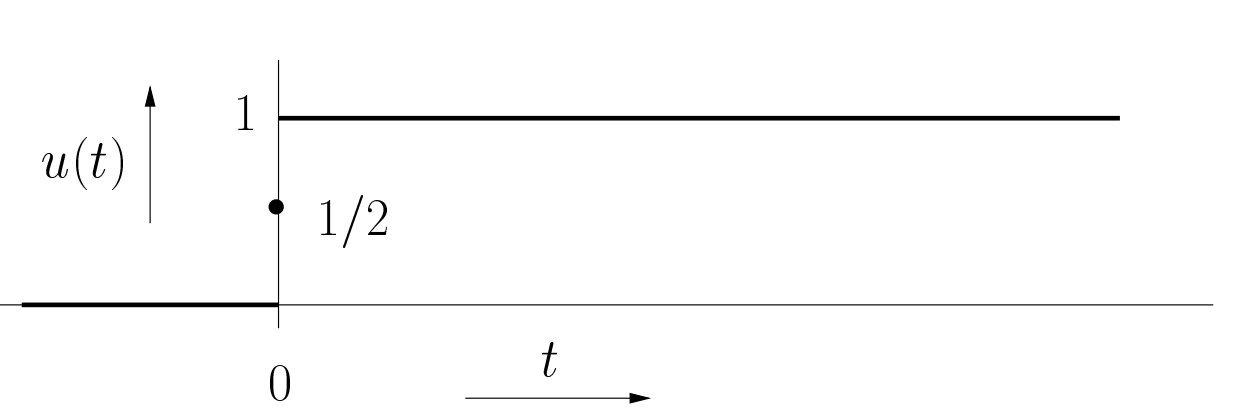
\includegraphics[width = 3.5cm]{include/Wichtige Funktionen/img/Sprungfunktion.png}}
    \\
    Signumfunktion
    \newline (Vorzeichenfunktion)
     &
    $\begin{cases}
         -1 \textrm{ für }  t<0,  \\
         0 \textrm{ für }  t = 0, \\
         1 \textrm{ für }  t >0.
       \end{cases}   $
     &
    $\frac{2}{j\omega}$
     &
    $sgn(t)$
     &
    \raisebox{-.5\height}{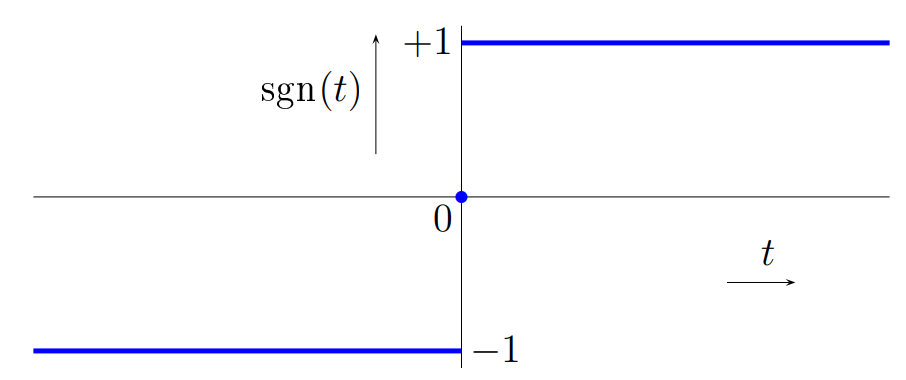
\includegraphics[width=3.5cm]{include/Wichtige Funktionen/img/Signumfunktion.png}}
    \\
    Rampenfunktion
     &
    $\begin{cases}
         0 \textrm{ für } t \leq 0, \\
         t \textrm{ für } t > 0.
       \end{cases}$
     &
    $\frac{1}{s^2}$
     &
    $r(t)$
     &
    \raisebox{-.5\height}{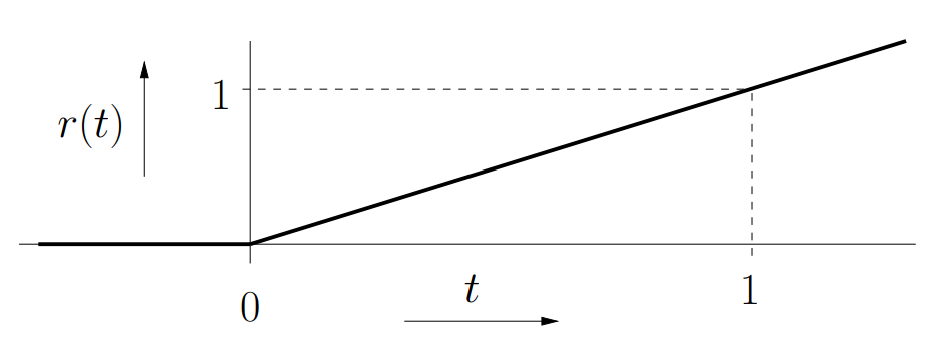
\includegraphics[width=3.5cm]{include/Wichtige Funktionen/img/Rampenfunktion.png}}
    \\
    Rechteckimpuls
     &
    $\begin{cases}
         1 \textrm{ für } |t| < a,           \\
         \frac{1}{2} \textrm{ für } |t| = a, \\
         0 \textrm{ für } |t| > a.
       \end{cases} $
     &
    $\frac{1}{s}- e^{-as}\frac{1}{s} $
     &
    $p_a(t), \beta(t)$
    \newline $\sigma(t+a)-\sigma(t-a)$
     &
    \raisebox{-.5\height}{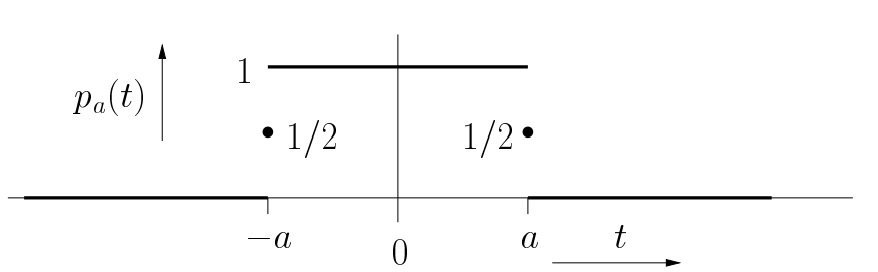
\includegraphics[width=3.5cm]{include/Wichtige Funktionen/img/Rechteckimpuls.png}}
    \\
    Dreieckimpuls
     &
    $\begin{cases}
         1 - \frac{|t|}{a} \textrm{ für } |t| < a \\
         0 \textrm{ für } |t| \geq a
       \end{cases}$
     &
    $sinc^2(\omega)$
     &
    $\Lambda(t)$
     &
    \raisebox{-.5\height}{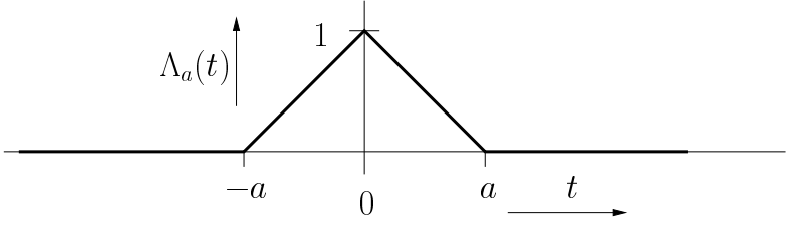
\includegraphics[width=3.5cm]{include/Wichtige Funktionen/img/Dreieckimpuls.png}}
    \\
    Sinc-Funktion
     &
    $\frac{sin(t)}{t}\; \forall t$
    \newline {\tiny $\lim _{t \to 0} sinc(t) = 1$}
    \newline {\tiny wenn normalisiert: $t \to \pi t$}
     &
    $\beta(\omega)$
    \newline{\tiny(Rechteckimpuls)}
     &
    sinc(t)
     &
    \raisebox{-.5\height}{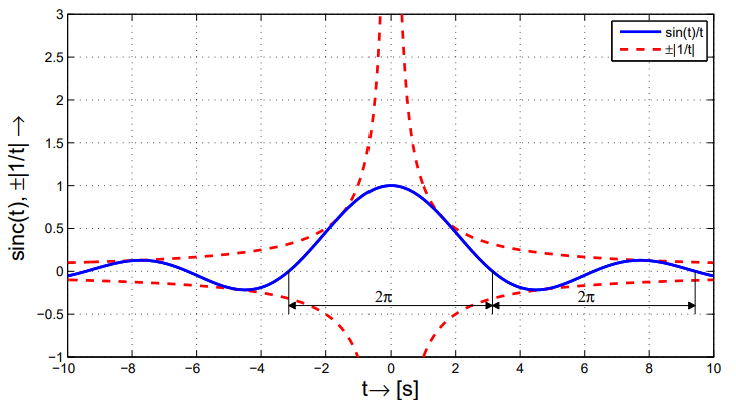
\includegraphics[width=3.5cm]{include/Wichtige Funktionen/img/SincFunktion.png}}
    \\
    \hline
  \end{tabular}
\section{Begriffe}
\begin{itemize}
      \item Prozess
            \begin{itemize}
                  \item Die Gesamtheit zusammenwirkender Vorgänge, welche durch
                        die Materie, Energie und Information
                        umgefort, transportiert und gespeichert wird.
            \end{itemize}

      \item System
            \begin{itemize}
                  \item Ist gegenüber der Umwelt abgegrenzt, hat Eingänge,
                        Ausgänge (und Zustand).
                  \item (LTI-/)LZI-Systeme: Lineare-ZeitInvariante Systeme
                        (Linearität gilt, System ist unabhängig von zeitlicher Verschiebung
                        --> DGL mit Konst. Koeff.)
            \end{itemize}

      \item Modell
            \begin{itemize}
                  \item Beschreibung von Systemen, wird genutzt für
                        Erklärung, Prognose, Gestaltung und Optimierung.
                  \item Es gibt kein "richtiges Modell",
                        ein Modell beschreibt ein System nur so genau wie nötig.
            \end{itemize}
      \item Modellieren
            \begin{itemize}
                  \item Teilsysteme erstellen und diese
                        in weitere Teilsysteme aufzutrennen.
                        So erhält man einfache Grundsysteme (Grundglieder),
                        welche sich einfach Mathematisch beschreiben lassen.
                        Zusätzlich kehern einige Teilsysteme in ihrer
                        Struktur oft wieder und können wiederverwendet werden.

                  \item Top-Down: System in Teilsysteme teilen
                  \item Bottom-Up: System aus Grundglieder aufbauen
            \end{itemize}
      \item Grundglieder
            \begin{itemize}
                  \item Kleinste Teilsysteme. Sie können weiter augeteilt werden in, siehe Abschnitt \nameref{Grundglieder}
            \end{itemize}
      \item Sprungantwort
            \begin{itemize}
                  \item Reaktion des Systems auf die Sprungfunktion. Siehe \refname{func}

            \end{itemize}
      \item Schrittantwort
      \item \begin{itemize}
                  \item Reaktion des Systems auf die Schrittfunktion. Siehe \refname{func}
            \end{itemize}
      \item Ausgleich
            \begin{itemize}
                  \item Prozesse ohne Ausgleich: Sprungantwort wächst Grenzenlos an
                  \item Prozess mit Ausgleich: Sprungantwort strebt endlichem Wert zu
            \end{itemize}

\end{itemize}


\subsection{Grundglieder}
\label{Grundglieder}
\begin{itemize}
      \item Statische Glieder(Systeme ohne Gedächtnis):
            Der Ausgang ist nur vom aktuellen Eingang abhängig.
            $y(t)=f(u(t))$
            \begin{itemize}
                  \item P-glied (Proportionalglied): Reagiert mit einem Faktor K auf den aktuellen Eingangswert.\\
                        $y = K \cdot u$
            \end{itemize}
      \item Dynamische Glieder (System mit Gedächtnis):
            Der Ausgang ist vom aktuellen sowie von vergangenen Eingängen Abhängig.
            Vergangene Eingänge werden im System als Zustand x(t) gespeichert.
            $y(t)=f(u(t),x(t))$ \\Können weiter unterteil werden in:
            \begin{itemize}
                  \item I-Glied (Integrierer):
                        Ausgangssignal ist Abhängig vom Integrierten Einganssignal, Allenfalls mit einem Faktor K multipliziert. \\
                        $y(t) = K \cdot \int \limits _{t=0} ^{t} u(\tau) d\tau + y(0)$ \\
                        $(\frac{dy(t)}{dt} =)$ \space $\dot{y}(t) = K \cdot u(t) $
                  \item Totzeitglied: Verzögert das Eingangssignal um die Totzeit $T_t$\\
                        $y(t) = u(t-T_t)$
                  \item PT\textsubscript{1}-Glied:
                        LZI-Übertragungsglied mit Proportionalem Übertragunsverhalten \\
                        und Verzögerung 1. Ordnung. (Bsp. Tiefpass 1.Ordnung als RC-Glied)

                  \item PT\textsubscript{2}-Glied
                        \begin{itemize}
                              \item Übertragungsglied mit Verhalten 2. Ordnung.
                              \item $T^2 \cdot \ddot{y}(t) + 2 \zeta T \cdot\dot{y}(t) + y(t) = K \cdot u(t)$
                        \end{itemize}
                  \item D-Glied(idealer Differenzierer)
                        \begin{itemize}
                              \item Bildet die Zeitliche Ableitung des Signals, mit einer Verstärkung K.
                              \item $y(t) = K \cdot \frac{du(t)}{dt} = K\cdot \dot{u}(t)$
                        \end{itemize}
                  \item DT$_1$-Glied
                        \begin{itemize}
                              \item Realiserbar, im Gegensatz zum theoretischen D-Glied.
                              \item $T \cdot \dot{y}(t) + y(t) = K \cdot \dot{u}(t)$
                        \end{itemize}
                  \item PI-, PD- PID-Glied (PDT$_1$ und PIDT$_1$)
                        \begin{itemize}
                              \item Werden häufig als Regler eingesetzt.
                              \item Name setzt sich aus den Aktiven Pfaden zusammen.
                                    \begin{itemize}
                                          \item P: Proportional
                                          \item I: integrierend
                                          \item D: Differenzierend
                                          \item P, I und D in Kombination sind Parallel
                                          \item T\textsubscript{1,2,t} bezieht sich auf die vorangehende Komponente.
                                    \end{itemize}
                              \item Berechnet sich aus Superposition der Teilantworten
                              \item $y(t) = A \cdot [K_P + K_I \cdot t + \frac{K_D}{T_C} \cdot e^{\frac{-t}{T_C}}]$
                        \end{itemize}
                  \item Lead-Glied, Lag-Glied, Lead-Lag-Glied
                        \begin{itemize}
                              \item Varianten von PDT\textsubscript{1}-Gliedern.
                              \item Unterscheiden sich im Vorzeichen von $K_P$ und $K_D$.
                        \end{itemize}

            \end{itemize}
\end{itemize}

% Needs Package: \usepackage{bm}
\section{LTI-Systeme}

$ y(t) = \mathcal{T}[x(t)]$

\begin{multicols}{2}
    \subsection*{Linearität und Zeitinvarianz}
    \begin{itemize}
        \item $\mathcal{T}[x_1(t) + x_2(t)] = y_1(t) + y_2(t)$
        \item $\mathcal{T}[k_a \cdot x(t)] = k_a \cdot y(t)$
        \item $\mathcal{T}[x(t-t_0) = y(t-t_0)]$
    \end{itemize}

    \subsection*{Kausalität}
    \begin{itemize}
        \item Jede Wirkung hat eine Ursache
        \item der Aktuelle y(t) Wert ist vom zukünftigen x(t) unabhängig
        \item Mathematische Systeme müssen nicht Kausal sein
        \item Physikalisch ist Kausalität ein Grundprinzip nach Newton
    \end{itemize}

    \subsection{Beschreibung von LTI Systemen}

    \subsubsection{Impulsantwort}
    Impulsfunktion $\delta(t)$ wird am Eingang des Systems angelegt,
    die Reaktion darauf am Ausgang nennt man die \textbf{Impulsantwort} \bm{$h(t)$}.
    Sie beschreibt ein LTI-System vollständig.

    $$ y(t) = \mathcal{T}[x(t)]
        = \int \limits _{-\infty} ^{infty} x(\tau) \cdot h(t-\tau)d\tau
        = x(t) * h(t)$$
    \subsubsection*{Kausalität}
    Bei einem Kausalen System ist $h(t) = 0$ für $t<0$

    \subsection*{Verzerrung}
    Verzerrung = Verformung des Eingangssignals (gefiltert, moduliert, gedämpft, entzerrt).
    Sie ist bei LTI Systemen \textbf{linear}.
    Eigenschaften:
    \begin{itemize}
        \item Amplitudenverzerrung:
              \begin{itemize}
                  \item $|H(\omega)|$ unkonstant
                  \item Spektralanteile $X(\omega)$ in $Y(\omega)$ nicht gleich gross
                  \item $Y(\omega)$ hat keine zusätzlichen Spektralanteile
              \end{itemize}
        \item Phasenverzerrung:
              \begin{itemize}
                  \item $\varphi(\omega)$ nicht linear zu $\omega$
                  \item Spektralanteile nach Frequenz zeitlich ungleich verzögert
                  \item Signal im Zeitbereich $x(t) \neq y(t)$
              \end{itemize}
    \end{itemize}
    \textbf{Verzerrungsfrei:} Ausgangssignal wird nur um einen Faktor $k_a$ skaliert
    oder um eine Zeit $t_d$ verzögert. somit gilt:
    \begin{itemize}
        \item Übertragungsfunktion: $H(\omega) = k_a \cdot e^{-j\omega z_d}$
        \item   Amplitudengang: $|H(\omega)| = k_a$
        \item  Phasengang: $\varphi_h(\omega) = -t_d \cdot \omega$
    \end{itemize}

    \subsubsection{Frequenzantwort}
    Die \textbf{Frequenzantwort} $\bm{H(\omega)}$ ist die Fouriertransformierte Impulsantwort.
    Sie ist eine komplexwertige dimensionslose Gewichstsfunktion.
    Auch sie beschreibt ein LTI-System vollständig.

    $$ Y(\omega) = X(\omega) \cdot H(\omega)$$

    \subsubsection*{Berechnung des Ausgangssignals}
\begin{enumerate}
   \item Fourier-Transformation:  $X(\omega) = \mathcal{F}[x(t)]$ 
   \item Berechnung in Frequenz  $Y(\omega) = X(\omega) \cdot H(\omega)$ 
   \item Rücktransformation:  $y(t) = \mathcal{F}^{-1}[Y(\omega)]$ 
\end{enumerate}


    \subsubsection*{Bezeichnungen}
    Übertragungsfunktion: $H(\omega)=|H(\omega)| \cdot e^{j\varphi_H(\omega)}$ \\
    Amplitudengang: $|H(\omega)|$ \\
    Phasengang: $\varphi_H(\omega)$ \\

    \subsubsection*{Filtereigenschaften}
    $Y(\omega) = X(\omega) \cdot H(\omega)$ \\
    $|Y(\omega)| = |X(\omega)| \cdot |H(\omega)|$ \\
    $\varphi_y(\omega) = \varphi_x(\omega) + \varphi_H(\varphi)$

    \subsubsection*{Filtertypen}
    \begin{itemize}
        \item Tiefpassfilter: Alle Frequenzen \textbf{grösser} als Eckfrequenz $\omega_c$ werden weggefiltert.
        \\ $H(\omega) = 0$ für $|\omega| > \omega_c$
        \\ Bandbreite: Von Frequenz 0 Hz bis Eckfrequenz.
        \item Hochpassfilter: Alle Frequenzen \textbf{kleiner} als Eckfrequenz $\omega_c$ werden weggefiltert.
        \\ $H(\omega) = 0$ für $|\omega| < \omega_c$
        \item Bandpassfilter: Alle Frequenzen \textbf{ausserhalb} der Eckfrequenzen $\omega_{c1,2}$ werden weggefiltert.
        \\ $H(\omega) = 0$ für $|\omega| < \omega_{c1}$  und $H(\omega) = 0$ für $|\omega| > \omega_{c2}$
        \\ Bandbreite: Von unterer bis zur oberen Eckfrequenz
        \item Bandsperre: Alle Frequenzen \textbf{innerhalb} der Eckfrequenzen $\omega_{c1,2}$ werden weggefiltert.
        \\ $H(\omega) = 0$ für $\omega_{c1} < |\omega| < \omega_{c2}$
        \item Quadraturfilter: Schiebt die Phase um $-90^{\circ}$.
        $H(\omega) = -j \cdot sign(\omega)$
    \end{itemize}

\end{multicols}



\section{Tabellen}
\subsection*{Blockschaltbilder-DIN}
\begin{tabular}{|c|c|c|c|c|}
      \hline
      \textbf{Summierer}                                       &
      \textbf{Differenzbilder}                                 &
      \textbf{Multiplizierer}                                  &
      \textbf{Proportionalglied}                               &
      \textbf{Integrierer}                                       \\
      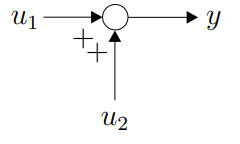
\includegraphics[width = 3cm]{img/Summierer.png}         &
      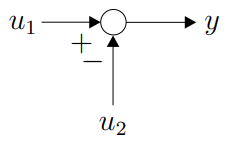
\includegraphics[width = 3cm]{img/Differenzbilder.png}   &
      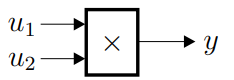
\includegraphics[width = 3cm]{img/Multiplizierer.png}    &
      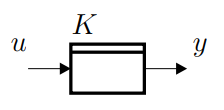
\includegraphics[width = 3cm]{img/Proportionalglied.png} &
      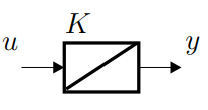
\includegraphics[width = 3cm]{img/Integrator.png}          \\
      \hline
      \textbf{Totzeitglied}                                    &
      \textbf{PT\textsubscript{1}-Glied}                       &
      \textbf{PT\textsubscript{2}-Glied}                       &
      \textbf{idealer Differenzierer}                          &
      \textbf{DT\textsubscript{1}-Glied}                         \\
      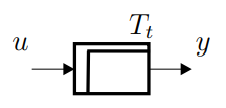
\includegraphics[width = 3cm]{img/Totzeitglied.png}      &
      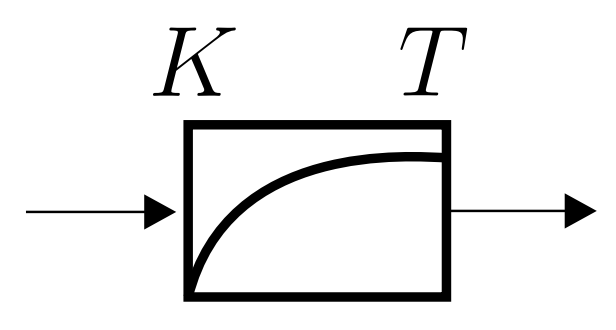
\includegraphics[width = 3cm]{img/PT1-Glied.png}         &
      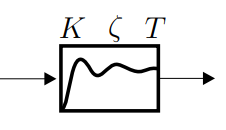
\includegraphics[width = 3cm]{img/PT2-Glied.png}         &
      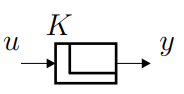
\includegraphics[width = 3cm]{img/D-Glied.png}           &
      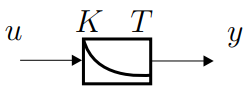
\includegraphics[width = 3cm]{img/DT-Glied.png}            \\
      \hline
\end{tabular}

\subsection*{Blockschaltbilder MatLab}
\begin{tabular}{|c|c|c|c|c|}
      \hline
      \textbf{Summierer}                                            &
      \textbf{Differenzbilder}                                      &
      \textbf{Konstante}                                            &
      \textbf{Proportionalglied}                                    &
      \textbf{Integrierer}                                            \\
      
\includegraphics[]{img/matlab/sum_block_icon.png}             &
      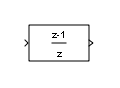
\includegraphics[]{img/matlab/difference_block_icon.png}      &
      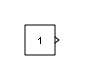
\includegraphics[]{img/matlab/constant_block_icon.png}        &
      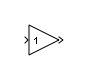
\includegraphics[]{img/matlab/gain_block_icon.png}            &
      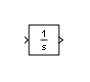
\includegraphics[]{img/matlab/integrator_block_icon.png}        \\
      \hline
      \textbf{Totzeitglied}                                         &
      \textbf{Differenzierer}                                       &
      \textbf{}                                                     &
      \textbf{}                                                     &
      \textbf{}                                                       \\
      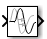
\includegraphics[]{img/matlab/transport_delay_block_icon.png} &
      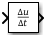
\includegraphics[]{img/matlab/derivative_block_icon.png}      &
      \\
      \hline
\end{tabular}
\end{document}
